% The ripple pencil over R and over F_7.
\documentclass[tikz,border=8pt]{standalone}
\usepackage{amsmath,amssymb}
\usetikzlibrary{arrows.meta}
\begin{document}
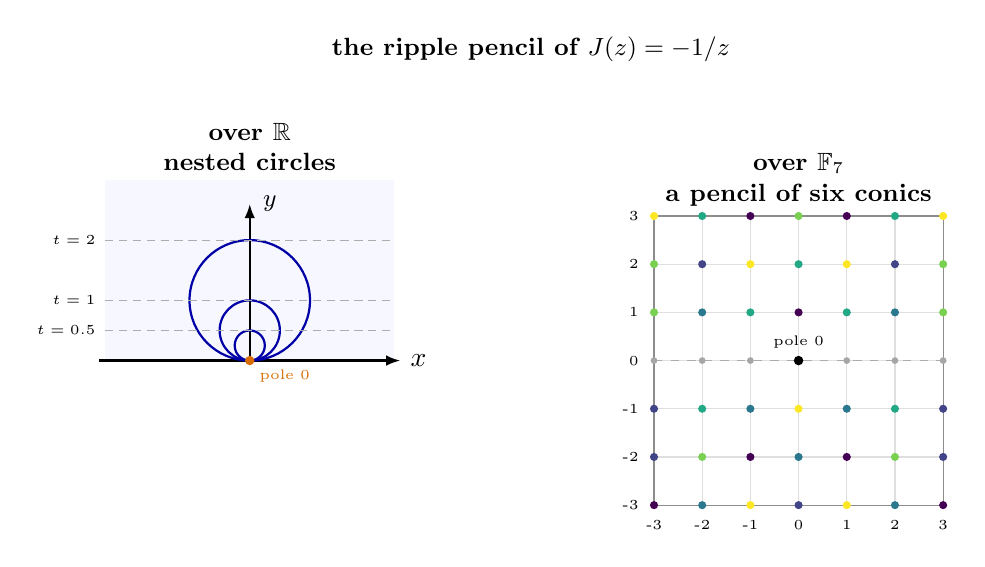
\begin{tikzpicture}[scale=0.85]
\definecolor{tA}{HTML}{440154}
\definecolor{tB}{HTML}{414487}
\definecolor{tC}{HTML}{2A788E}
\definecolor{tD}{HTML}{22A884}
\definecolor{tE}{HTML}{7AD151}
\definecolor{tF}{HTML}{FDE725}
\begin{scope}[xshift=-4.2cm,scale=0.9]
  \fill[blue!3] (-2.4,0) rectangle (2.4,3.0);
  \draw[-{Latex[length=1.8mm]}, thick] (-2.5,0)--(2.5,0) node[right] {$x$};
  \draw[-{Latex[length=1.8mm]}, thick] (0,0)--(0,2.6);
  \foreach \t/\r in {0.5/1.0,1/0.5,2/0.25} {
    \draw[blue!65!black, thick] (0,\r) circle (\r);
  }
  \foreach \t in {0.5,1,2} {
    \draw[gray!65, densely dashed] (-2.4,\t)--(2.4,\t);
    \node[font=\tiny,left] at (-2.4,\t) {$t=\t$};
  }
  \fill[orange!85!black] (0,0) circle (2.2pt) node[below right,font=\tiny] {pole $0$};
  \node[font=\small,right] at (0.06,2.6) {$y$};
  \node[font=\small\bfseries,align=center] at (0,3.55) {over $\mathbb R$\\ nested circles};
\end{scope}
\begin{scope}[xshift=4.0cm,scale=0.72]
  \draw[gray!25] (-3,-3) grid (3,3);
  \draw[black!45] (-3,-3) rectangle (3,3);
  \foreach \x in {-3,...,3} {\node[font=\tiny,below] at (\x,-3.12) {\x};}
  \foreach \y in {-3,...,3} {\node[font=\tiny,left] at (-3.12,\y) {\y};}
  \fill[tA] (-3,-3) circle (2.4pt);
  \fill[tA] (-1,-2) circle (2.4pt);
  \fill[tA] (-1,3) circle (2.4pt);
  \fill[tA] (0,1) circle (2.4pt);
  \fill[tA] (1,-2) circle (2.4pt);
  \fill[tA] (1,3) circle (2.4pt);
  \fill[tA] (3,-3) circle (2.4pt);
  \fill[tB] (-3,-2) circle (2.4pt);
  \fill[tB] (-3,-1) circle (2.4pt);
  \fill[tB] (-2,2) circle (2.4pt);
  \fill[tB] (0,-3) circle (2.4pt);
  \fill[tB] (2,2) circle (2.4pt);
  \fill[tB] (3,-2) circle (2.4pt);
  \fill[tB] (3,-1) circle (2.4pt);
  \fill[tC] (-2,-3) circle (2.4pt);
  \fill[tC] (-2,1) circle (2.4pt);
  \fill[tC] (-1,-1) circle (2.4pt);
  \fill[tC] (0,-2) circle (2.4pt);
  \fill[tC] (1,-1) circle (2.4pt);
  \fill[tC] (2,-3) circle (2.4pt);
  \fill[tC] (2,1) circle (2.4pt);
  \fill[tD] (-2,-1) circle (2.4pt);
  \fill[tD] (-2,3) circle (2.4pt);
  \fill[tD] (-1,1) circle (2.4pt);
  \fill[tD] (0,2) circle (2.4pt);
  \fill[tD] (1,1) circle (2.4pt);
  \fill[tD] (2,-1) circle (2.4pt);
  \fill[tD] (2,3) circle (2.4pt);
  \fill[tE] (-3,1) circle (2.4pt);
  \fill[tE] (-3,2) circle (2.4pt);
  \fill[tE] (-2,-2) circle (2.4pt);
  \fill[tE] (0,3) circle (2.4pt);
  \fill[tE] (2,-2) circle (2.4pt);
  \fill[tE] (3,1) circle (2.4pt);
  \fill[tE] (3,2) circle (2.4pt);
  \fill[tF] (-3,3) circle (2.4pt);
  \fill[tF] (-1,-3) circle (2.4pt);
  \fill[tF] (-1,2) circle (2.4pt);
  \fill[tF] (0,-1) circle (2.4pt);
  \fill[tF] (1,-3) circle (2.4pt);
  \fill[tF] (1,2) circle (2.4pt);
  \fill[tF] (3,3) circle (2.4pt);
  \draw[gray!65, dashed] (-3,0)--(3,0);
  \fill[gray!70] (-3,0) circle (2.0pt);
  \fill[gray!70] (-2,0) circle (2.0pt);
  \fill[gray!70] (-1,0) circle (2.0pt);
  \fill[gray!70] (1,0) circle (2.0pt);
  \fill[gray!70] (2,0) circle (2.0pt);
  \fill[gray!70] (3,0) circle (2.0pt);
  \fill[black] (0,0) circle (2.8pt);
  \node[font=\tiny] at (0,0.38) {pole $0$};
  \node[font=\small\bfseries,align=center] at (0,3.75) {over $\mathbb F_7$\\ a pencil of six conics};
\end{scope}
\node[font=\small\bfseries] at (0,4.65) {the ripple pencil of $J(z)=-1/z$};
\end{tikzpicture}
\end{document}